\chapter{Opdracht week 4}

\section{Toepassing 1}


\subsection{Relatie SWOT}

Een belangrijk punt voor ons bedrijf is goede communicatie.
Wij willen duidelijk zijn tegenover de gebruikers van onze service.
Zo willen wij een betrouwbare omgeving creëren voor iedereen die onze services gebruikt.
Een goede manier om deze duidelijkheid te verbeteren en
om onze gebruikers beter te kunnen helpen is het hanteren van een Customer Relation Management systeem. 

\subsection{Uitbreidingsplan}

\subsubsection{Doel}

Hiermee slaan wij de gegevens op van elk bedrijf dat zich bij ons registreert,
met welke bedrijven zij contact opnemen,
hoe vaak een bedrijf actief is en nog veel meer.
Wij kunnen hier gebruik van maken door bijvoorbeeld te kijken van welke functies op de site ondernemingen vaak gebruik maken.
Zijn grotere bedrijven alleen op zoek naar andere grotere bedrijven, of kijken ze ook naar zzp’ers?
Zo kunnen wij een gedetailleerd overzicht krijgen over hoe onze service gebruikt wordt en door wie.
Op basis van deze informatie kunnen wij ingrijpen waar nodig.

\subsubsection{Impact}

Zodra een bedrijf vraagt om hulp of een klacht heeft over een ander bedrijf of
over een functie kunnen wij direct kijken of de klacht van het bedrijf te maken heeft met de recente historie van de desbetreffende ondernemingen of de klacht dus wel geloofwaardig is.
Hiermee versterken wij ons doel om een duidelijke regelgeving te hanteren op de site die zonder uitzonderingen nageleefd moet worden.
Door naar de geschiedenis van een bedrijf op onze site te kijken kunnen wij zien of zij wel conform de regels handelen.
Wij willen compleet transparant zijn dus wellicht is er zelfs een mogelijkheid waarbij andere bedrijven de samenwerkingsgeschiedenis kunnen zien van een geregistreerd bedrijf.
Uiteraard wordt precies vermeld welke informatie van de gebruikers wordt opgeslagen en waarom deze wordt opgeslagen.

\subsubsection{Omschrijving}

\section{Toepassing 2}

Gezien we een handjevol competente ICT Beheerders in de groep hebben,
is het normaal om de benodigde ICT-gerelateerde services zelf te beheren.
Omdat er een grote kans is dat er meerdere servers benodigd zullen zijn,
is het belangrijk om een goede basis te hebben.

\subsection{Relatie SWOT}

Het bedrijf is gefocused op snelle communicatie,
hiervoor is een stabiel platform erg belangrijk.
Dit systeem zorgt er ook voor dat systeembeheerders meer 'agile' kunnen werken.
Dit zorgt ervoor dat we als klein bedrijf wendbaar blijven.

\subsection{Uitbreidingsplan}

\subsubsection{Doel}

Dit systeem moet er voor zorgen dat het beheren van alle servers in het bedrijf
makkelijker en beter schaalbaar wordt door een deel ervan te automatiseren.
Daarom is dit systeem een groot voordeel voor systeembeheerders binnen het bedrijf.

Gezien de website van het bedrijf op Linux zal worden gedraaid,
zal dit systeem ook op Linux draaien.
Om ervoor te zorgen dat er snel nieuwe servers op kunnen worden gezet,
word er een hypervisor ingezet samen met een configuration management server.

\subsubsection{Impact}

Voor het implementeren van dit systeem zal er minimaal 1 systeembeheerder nodig zijn.
Voor een enkele systeembeheerder met kennis van zoiets dergelijks
zal het implementeren hiervan ongeveer 2-3 weken kosten, sprekende uit ervaring
van 1 van systeembeheerders.

\subsubsection{Omschrijving}
{\bf Systeemontwerpen, wireframes, designs}


\section{Toepassing 3}

Als eerste werd er natuurlijk gedacht aan het originele idee,
een website waarop services gedeeld en ingehuurd worden.

\subsection{Relatie SWOT}
{\bf Hoe zijn we op dit idee gekomen, hoe is dit gerelateerd}

\subsection{Uitbreidingsplan}

\subsubsection{Doel}
{\bf Bedoeling met het systeem,
  welke partijen hebben er mee te maken}





\subsubsection{Functioneel ontwerp}

Digitale benodigdheden:

\begin{itemize}
\item
  Zoekmachine
  \begin{itemize}
  \item
    Optie om naar bedrijven te zoeken
    \begin{itemize}
    \item
      Filteren op soort bedrijf
    \end{itemize}
  \item
    Optie om naar services te zoeken
  \end{itemize}
\item  
  Een bedrijf moet een verzoek kunnen plaatsen waarin vermeld wordt naar
  wat voor service zij op zoek zijn, hier moet op gereageerd kunnen
  worden
\item
  Bij het aanmelden van een bedrijf moet er een pagina komen voor het
  desbetreffende bedrijf
  
  \begin{itemize}
  \item
    Hier moet informatie staan over het bedrijf,
    zoals de aangeboden services en de locaties,
    dit moet zelf toegevoegd kunnen worden.
    Dit kan in de vorm van wat tekst,
    foto’s of zelfs een introductievideo.
  \item
    Er moet een mogelijkheid zijn om contact op te nemen met het bedrijf,
    dit kan via de site, maar er kunnen ook telefoonnummers of
    e-mails neergezet worden.
  \item
    Recensies over het bedrijf moeten weergegeven worden en
    gefilterd kunnen worden op bijvoorbeeld hoge naar lage waardering of
    hoge naar lage behulpzaamheid.
  \item
    Als er wordt gekozen om het bekend te maken kunnen er vorige
    samenwerkingen met andere bedrijven staan zodat de geschiedenis van
    een bedrijf wat beter in beeld komt.
  \item
    Wellicht kan elke bedrijfspagina een soort nieuwsbord hebben
    waar zij updates en mededelingen kunnen plaatsen over hun bedrijf.
  \end{itemize}

  \item
    Voorpagina met aanbevelingen voor contacten en/of updates over de
    website zelf.
  
  \begin{itemize}
  \item
    Gebaseerd op recente activiteiten van het bedrijf.
  \item
    Is er niet ingelogd dan worden simpelweg de populairste
    bedrijven laten zien in plaats van aanbevolen bedrijven.
  \end{itemize}
\end{itemize}

Mogelijkheid om na een samenwerking een soort recensie te plaatsen
over het andere bedrijf. Een recensie kan uiteraard alleen geschreven
worden na een geregistreerde samenwerking. Misschien kan er een
mogelijkheid zijn voor de lezers van de recensies om te beoordelen of
de recensie behulpzaam was, zo kunnen slecht geschreven recensies
minder aandacht krijgen.

\subsubsection{Technisch Ontwerp}





\subsubsection{Impact}
{\bf Wat is er nodig, wat gebeurt er met het bedrijf}

Hieronder is een simpel voorbeeld van de onderliggende architectuur.

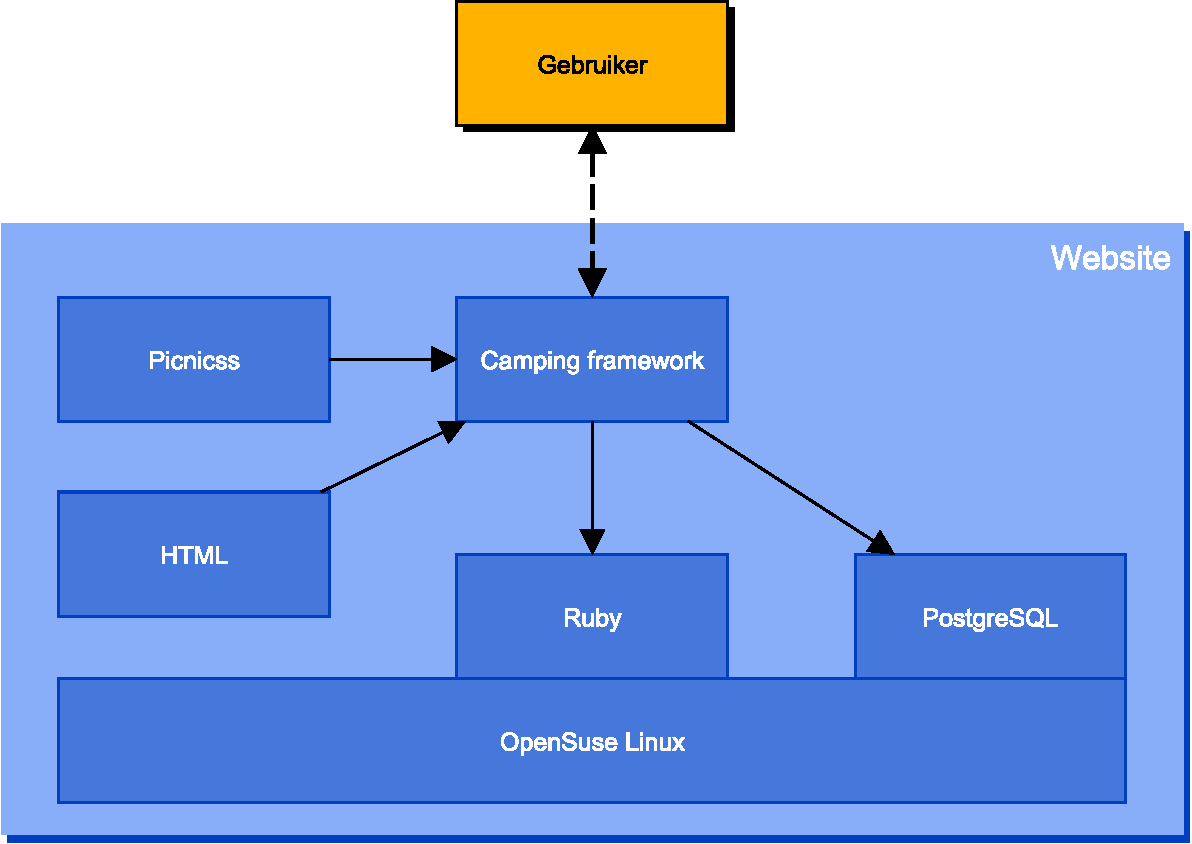
\includegraphics[width=\textwidth]{img/websiteArchitecture}

\subsubsection{Omschrijving}
{\bf Systeemontwerpen, wireframes, designs}